\documentclass[tikz, border=0pt, multi=tikzpicture]{standalone}
\usepackage[utf8]{inputenc}
\usepackage[T1]{fontenc}

% --- Typography: Modern Tech Look ---
\usepackage{helvet}
\usepackage[scale=1]{tgheros}
\renewcommand{\familydefault}{\sfdefault}
\usepackage{lmodern} 

\usepackage{pifont}
\usepackage{fontawesome5}
\usepackage[hidelinks]{hyperref}

% --- TikZ Libraries ---
\usetikzlibrary{
    shapes.geometric, 
    arrows.meta, 
    positioning, 
    fit, 
    calc, 
    shadows.blur, 
    backgrounds, 
    decorations.pathmorphing, 
    decorations.text, 
    patterns, 
    shapes.symbols, 
    matrix, 
    decorations.pathreplacing, 
    chains, 
    scopes
}

% --- Colors ---
\definecolor{bgWhite}{RGB}{255, 255, 255}
\definecolor{bgOffWhite}{RGB}{248, 250, 252}   % Slate 50
\definecolor{textBlack}{RGB}{15, 23, 42}       % Slate 900
\definecolor{textGray}{RGB}{71, 85, 105}       % Slate 600
\definecolor{primaryBlue}{RGB}{37, 99, 235}    % Blue 600
\definecolor{accentTeal}{RGB}{13, 148, 136}    % Teal 600
\definecolor{alertRed}{RGB}{220, 38, 38}       % Red 600
\definecolor{codeBg}{RGB}{30, 41, 59}          % Slate 800
\definecolor{borderGray}{RGB}{226, 232, 240}   % Slate 200
\definecolor{success}{RGB}{34, 197, 94}        % Green 500
\definecolor{warning}{RGB}{245, 158, 11}       % Amber 500

% Architecture Specific
\definecolor{archPrimary}{RGB}{0, 122, 204}
\definecolor{archSecondary}{RGB}{45, 45, 45}
\definecolor{archAccent}{RGB}{255, 140, 0}

% --- Layout ---
\def\slideW{16}
\def\slideH{20}
\def\margin{1.5}
\def\contentW{13}

% --- Styles ---
\tikzset{
    slide/.style={
        rectangle,
        fill=bgWhite,
        minimum width=\slideW cm,
        minimum height=\slideH cm,
        anchor=south west
    },
    h1/.style={
        font=\bfseries\Huge,
        text=textBlack,
        align=flush left,
        text width=\contentW cm,
        anchor=north west
    },
    h2/.style={
        font=\bfseries\huge,
        text=primaryBlue,
        align=flush left,
        text width=\contentW cm,
        anchor=north west
    },
    body/.style={
        font=\Large,
        text=textGray,
        align=flush left,
        text width=\contentW cm,
        anchor=north west,
        inner sep=0pt
    },
    card/.style={
        rectangle,
        rounded corners=12pt,
        fill=bgWhite,
        draw=borderGray,
        line width=1pt,
        blur shadow={shadow blur steps=5, shadow opacity=15},
        inner sep=15pt,
        align=flush left
    },
    artifact/.style={
        rectangle,
        rounded corners=4pt,
        fill=bgOffWhite,
        draw=textGray!50,
        dashed,
        font=\ttfamily\tiny,
        align=left,
        inner sep=4pt
    },
    % Architecture Diagram Styles
    basic/.style={
        rectangle, 
        rounded corners=6pt, 
        minimum width=3.5cm, 
        minimum height=1.5cm, 
        text centered, 
        draw=none, 
        fill=white,
        blur shadow={shadow blur steps=5, shadow opacity=10},
        font=\sffamily\small
    },
    module/.style={
        basic,
        draw=archPrimary,
        line width=1.2pt,
        fill=archPrimary!5
    },
    external/.style={
        basic,
        draw=archSecondary,
        line width=1.2pt,
        fill=archSecondary!5,
        dashed
    },
    database/.style={
        cylinder, 
        shape border rotate=90, 
        aspect=0.25, 
        minimum width=2.5cm, 
        minimum height=2cm, 
        text centered, 
        draw=archAccent, 
        line width=1.2pt,
        fill=archAccent!5, 
        blur shadow={shadow blur steps=5},
        font=\sffamily\small
    },
    archConnector/.style={
        ->, 
        thick, 
        draw=archSecondary!80,
        rounded corners=5pt,
        -{Latex}
    },
    connector/.style={
        ->, 
        thick, 
        draw=textGray, 
        rounded corners=5pt,
        -{Latex[scale=1.2]}
    },
    archBox/.style={ 
        rectangle, 
        rounded corners=5pt, 
        minimum width=3.5cm, 
        minimum height=1.2cm, 
        text centered, 
        draw=borderGray, 
        fill=bgWhite,
        font=\bfseries\small,
        blur shadow={shadow opacity=10}
    },
    processNode/.style={
        rectangle,
        rounded corners=6pt,
        minimum width=3.5cm, 
        minimum height=1.2cm, 
        text centered, 
        font=\bfseries\small, 
        draw=borderGray, 
        fill=bgWhite, 
        blur shadow={shadow opacity=10}
    }
}

\begin{document}

% =================================================================================
% SLIDE 1: HOOK (Honest & Open Source)
% =================================================================================
\begin{tikzpicture}
    \useasboundingbox (0,0) rectangle (\slideW, \slideH);
    \node[slide] at (0,0) {};
    
    % Background
    \draw[step=2cm, textGray!5, thin] (0,0) grid (\slideW, \slideH);
    \shade[top color=bgWhite, bottom color=primaryBlue!5] (0,0) rectangle (\slideW, \slideH);
    
    % Top Badge
    \node[fill=textBlack, text=bgWhite, rounded corners=15pt, inner sep=8pt, anchor=north east, font=\bfseries\small, blur shadow] at (15, 19) {
        \href{https://github.com/Om7035/Sentinel-The-Self-Healing-Knowledge-Graph}{
            \faGithub\ 100\% OPEN SOURCE
        }
    };
    \node[anchor=north east, font=\tiny\ttfamily, text=textGray] at (15, 18.3) {
        github.com/Om7035/Sentinel
    };
    
    % Main Visual
    \begin{scope}[shift={(8, 11)}]
        \fill[primaryBlue, opacity=0.1] (0,0) circle (3.8cm);
        \draw[primaryBlue, opacity=0.4, dashed, thick] (0,0) circle (3.5cm);
        \node[scale=5, text=primaryBlue] at (0,0) {\faShield*};
        \node[scale=2, text=bgWhite] at (0,0.2) {\faCheck};
        
        \node[fill=bgWhite, draw=borderGray, circle, inner sep=8pt, blur shadow] at (30:4cm) {\faDatabase};
        \node[fill=bgWhite, draw=borderGray, circle, inner sep=8pt, blur shadow] at (150:4cm) {\faGlobe};
        \node[fill=bgWhite, draw=borderGray, circle, inner sep=8pt, blur shadow] at (270:4cm) {\faClock};
    \end{scope}
    
    % Text
    \node[anchor=north, align=center] at (8, 17) {
        \fontsize{24}{28}\selectfont \textbf{Is Your RAG Data Stale?}\\[0.5em]
        \fontsize{18}{22}\selectfont \textcolor{textGray}{Meet the self-healing solution.}
    };
    
    \node[anchor=south, align=center] at (8, 3) {
        \fontsize{40}{45}\selectfont \textbf{\textcolor{primaryBlue}{SENTINEL}}\\[0.5em]
        \fontsize{20}{24}\selectfont \textbf{The Self-Healing}\\[0.2em]
        \fontsize{20}{24}\selectfont \textbf{Knowledge Graph}
    };
    
    \node[anchor=south, text=textGray, font=\small] at (8, 2.5) {
        Built for developers to create reliable, self-healing RAG pipelines.
    };

    % Library Mention
    \node[fill=codeBg, draw=borderGray, rounded corners=8pt, inner sep=12pt, anchor=south, blur shadow] at (8, 1.0) {
        \ttfamily\color{bgWhite}\Large \textbf{> pip install sentinel-core}
    };
    
    \node[anchor=south east, text=textGray!50, font=\small] at (15.5, 0.5) {1/13};
\end{tikzpicture}

% =================================================================================
% SLIDE 2: THE PROBLEM (Refined & Factual)
% =================================================================================
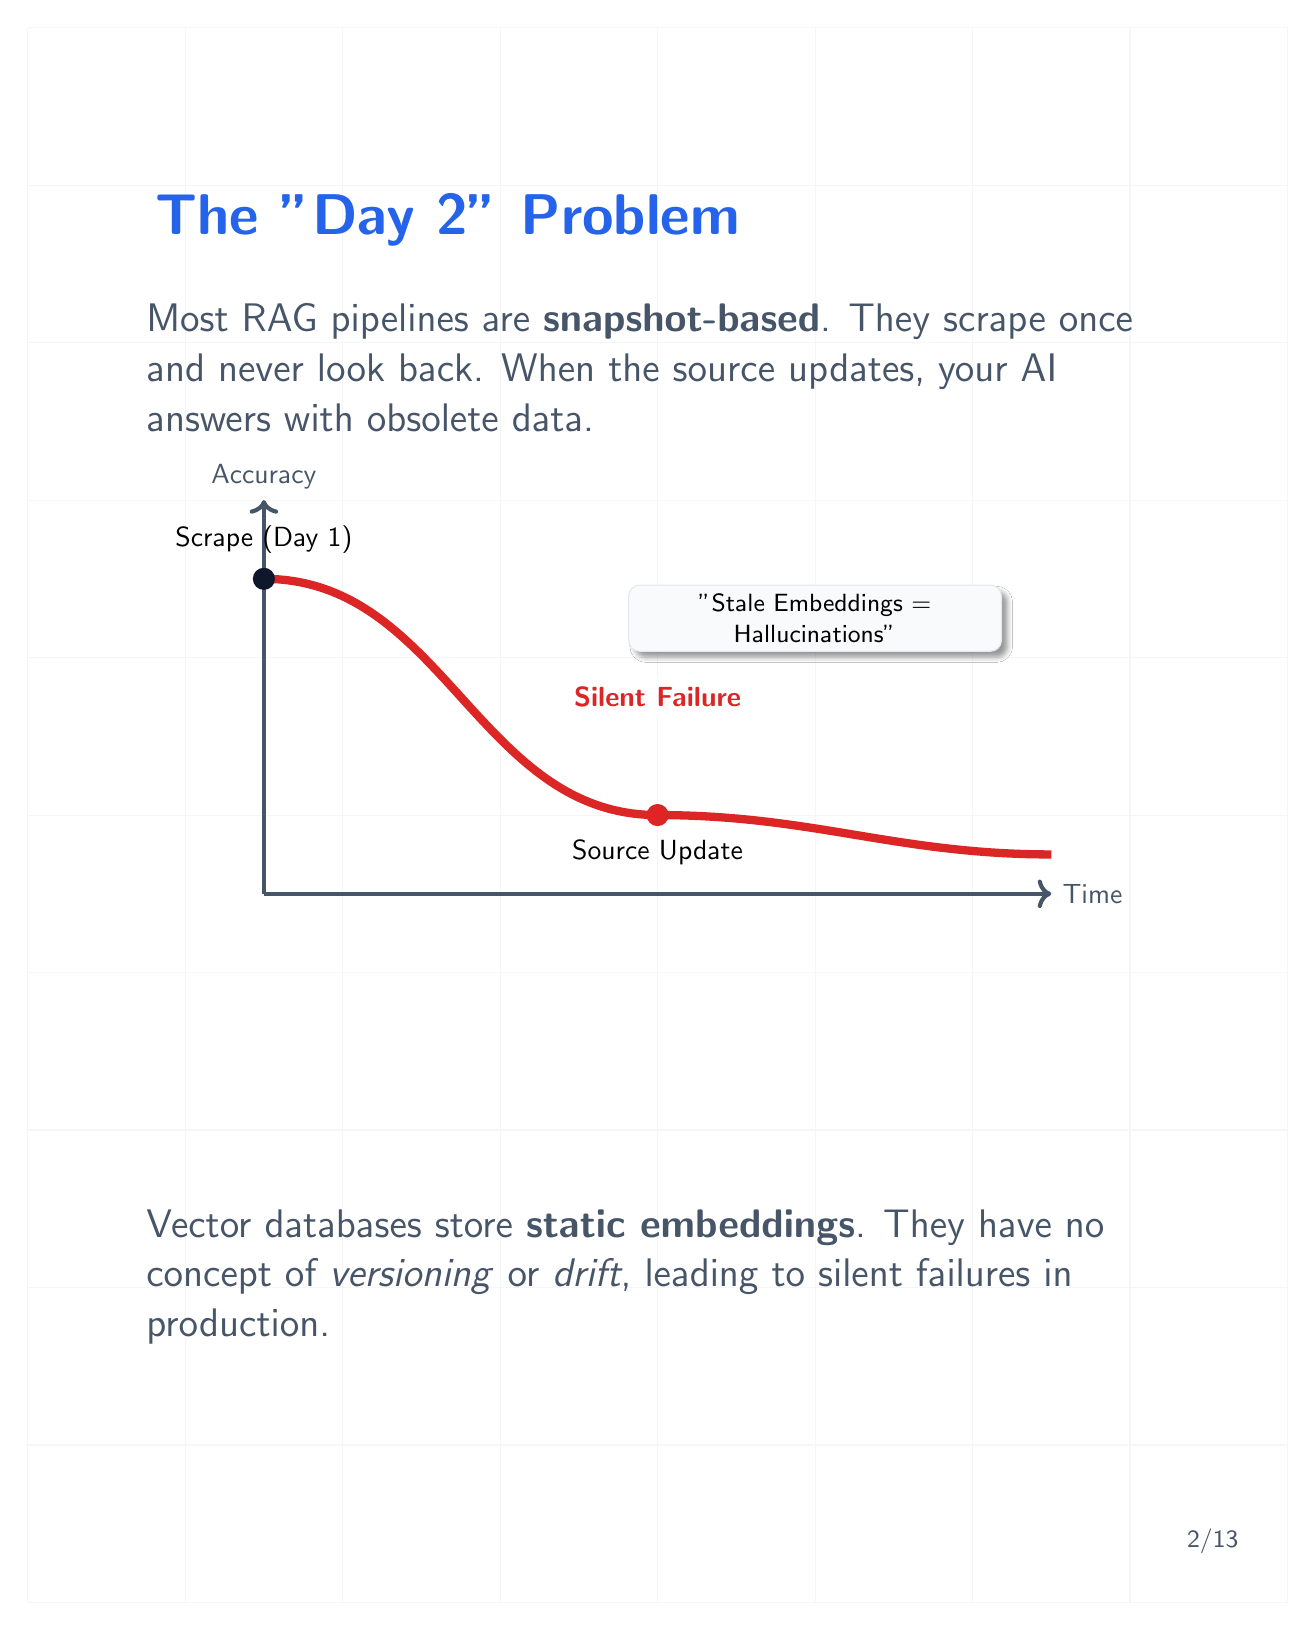
\begin{tikzpicture}
    \useasboundingbox (0,0) rectangle (\slideW, \slideH);
    \node[slide] at (0,0) {};
    \draw[step=2cm, textGray!5, thin] (0,0) grid (\slideW, \slideH);
    
    \node[h2] at (\margin, 18) {The "Day 2" Problem};
    
    \node[body] at (\margin, 16.5) {
        Most RAG pipelines are \textbf{snapshot-based}. They scrape once and never look back. When the source updates, your AI answers with obsolete data.
    };
    
    % Visual: Timeline of Decay
    \begin{scope}[shift={(8, 9)}] 
        \draw[->, line width=1.5pt, textGray] (-5,0) -- (5,0) node[right] {Time};
        \draw[->, line width=1.5pt, textGray] (-5,0) -- (-5,5) node[above] {Accuracy};
        
        % Curve
        \draw[alertRed, line width=3pt] (-5,4) to[out=0, in=180] (0,1) to[out=0, in=180] (5,0.5);
        \node[text=alertRed, font=\bfseries, fill=bgWhite] at (0, 2.5) {Silent Failure};
        
        % Points
        \fill[textBlack] (-5,4) circle (4pt);
        \node[above] at (-5,4.2) {Scrape (Day 1)};
        
        \fill[alertRed] (0, 1) circle (4pt);
        \node[below] at (0, 0.8) {Source Update};
        
        \node[text width=4.5cm, align=center, font=\small, fill=bgOffWhite, draw=borderGray, rounded corners, blur shadow] at (2, 3.5) {
            "Stale Embeddings =\\ Hallucinations"
        };
    \end{scope}
    
    \node[body, at={(\margin, 5)}] {
        Vector databases store \textbf{static embeddings}. They have no concept of \textit{versioning} or \textit{drift}, leading to silent failures in production.
    };
    
    \node[anchor=south east, text=textGray, font=\small] at (15.5, 0.5) {2/13};
\end{tikzpicture}

% =================================================================================
% SLIDE 3: THE SENTINEL LOOP (High Level Solution)
% =================================================================================
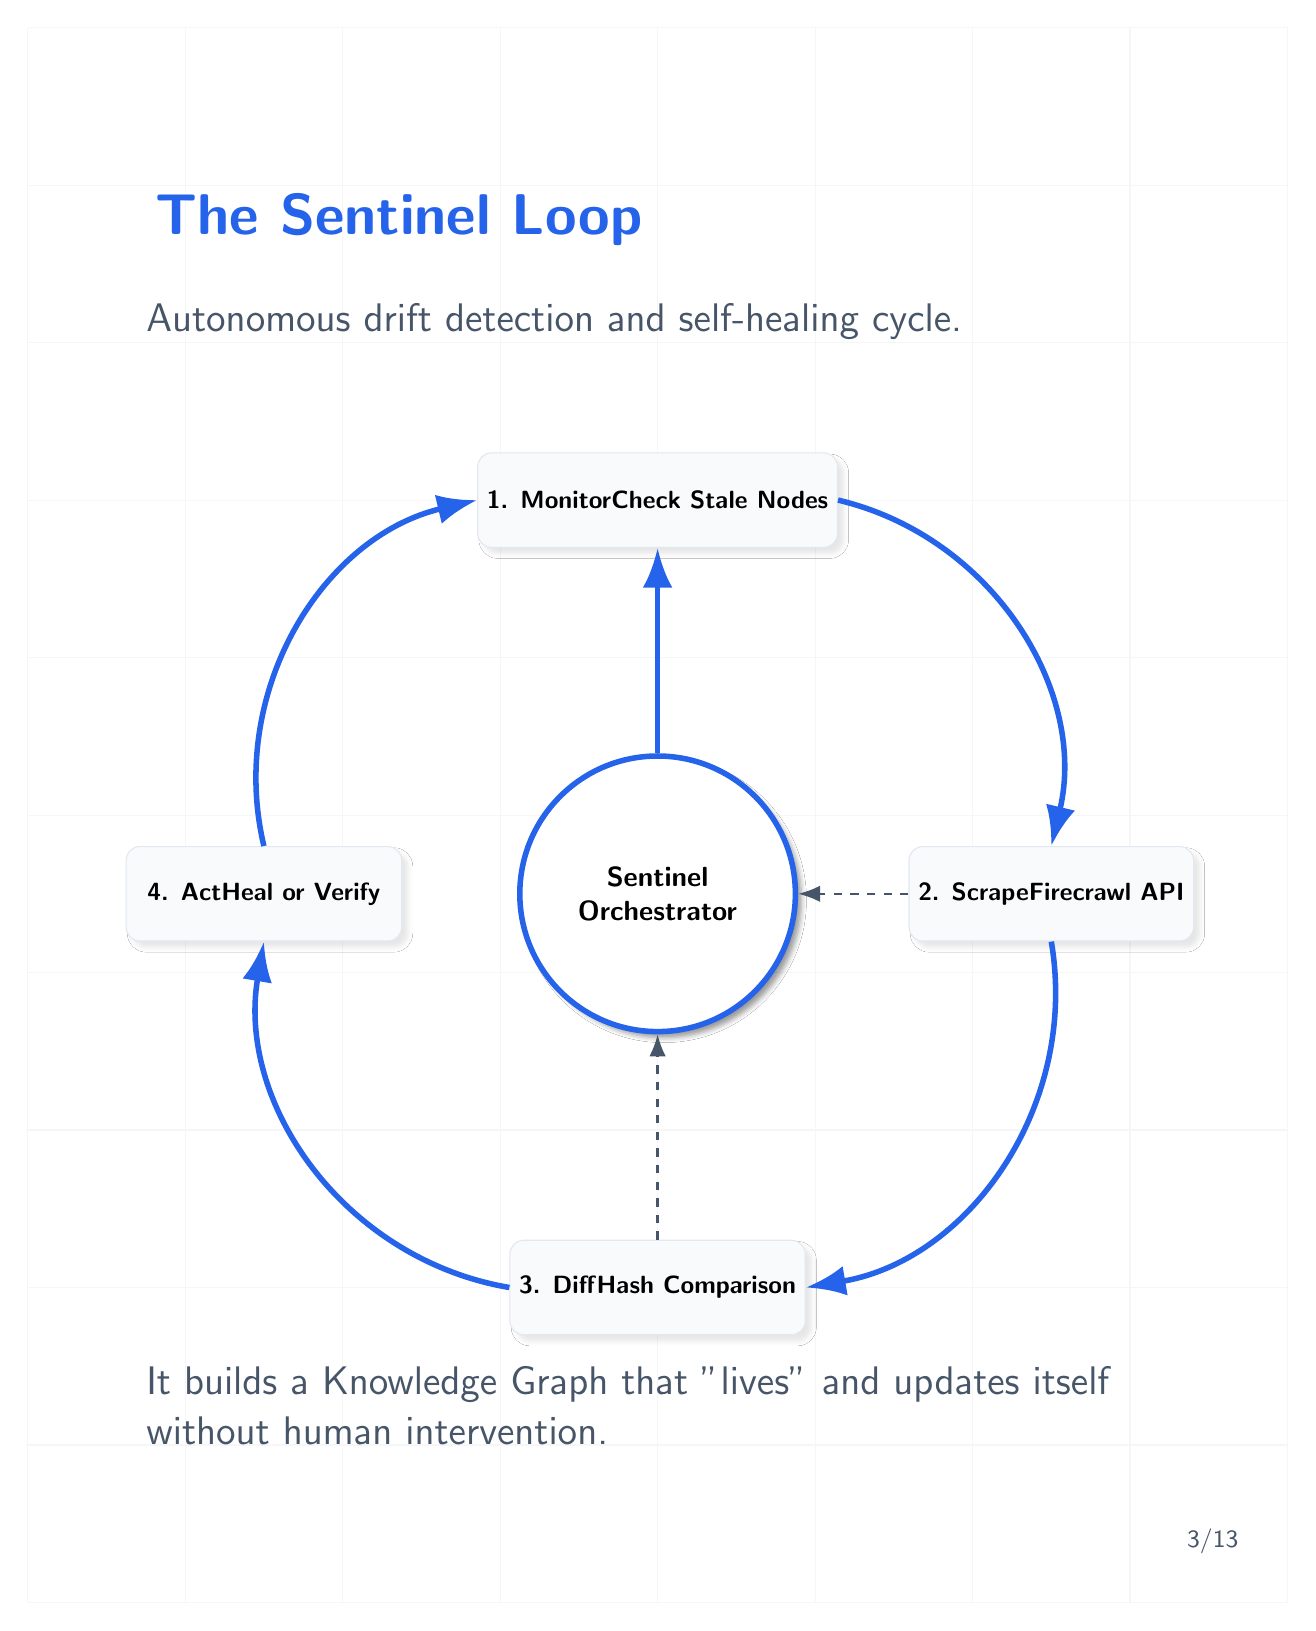
\begin{tikzpicture}
    \useasboundingbox (0,0) rectangle (\slideW, \slideH);
    \node[slide] at (0,0) {};
    \draw[step=2cm, textGray!5, thin] (0,0) grid (\slideW, \slideH);
    
    \node[h2] at (\margin, 18) {The Sentinel Loop};
    \node[body] at (\margin, 16.5) {
        Autonomous drift detection and self-healing cycle.
    };
    
    % Diagram: The Sentinel Loop
    \begin{scope}[shift={(8, 9)}]
        % Central Hub
        \node[circle, fill=bgWhite, draw=primaryBlue, line width=2pt, minimum size=3.5cm, align=center, blur shadow] (core) at (0,0) {\textbf{Sentinel}\\\textbf{Orchestrator}};

        % Outer Nodes
        \node[archBox, fill=bgOffWhite] (monitor) at (0, 5) {{\textbf{1. Monitor}\\ \small Check Stale Nodes}};
        \node[archBox, fill=bgOffWhite] (scrape) at (5, 0) {{\textbf{2. Scrape}\\ \small Firecrawl API}};
        \node[archBox, fill=bgOffWhite] (diff) at (0, -5) {{\textbf{3. Diff}\\ \small Hash Comparison}};
        \node[archBox, fill=bgOffWhite] (act) at (-5, 0) {{\textbf{4. Act}\\ \small Heal or Verify}};

        % Paths (Clockwise)
        \draw[connector, primaryBlue, line width=2pt] (core) -- (monitor);
        \draw[connector, primaryBlue, line width=2pt] (monitor) to[bend left=45] (scrape);
        \draw[connector, primaryBlue, line width=2pt] (scrape) to[bend left=45] (diff);
        \draw[connector, primaryBlue, line width=2pt] (diff) to[bend left=45] (act);
        \draw[connector, primaryBlue, line width=2pt] (act) to[bend left=45] (monitor);
        
        % Inner connections to Core
        \draw[connector, dashed, textGray] (scrape) -- (core);
        \draw[connector, dashed, textGray] (diff) -- (core);
    \end{scope}
    
    \node[body, at={(\margin, 3)}] {
        It builds a Knowledge Graph that "lives" and updates itself without human intervention.
    };
    
    \node[anchor=south east, text=textGray, font=\small] at (15.5, 0.5) {3/13};
\end{tikzpicture}

% =================================================================================
% SLIDE 4: ARCHITECTURE (Technical Deep Dive)
% =================================================================================
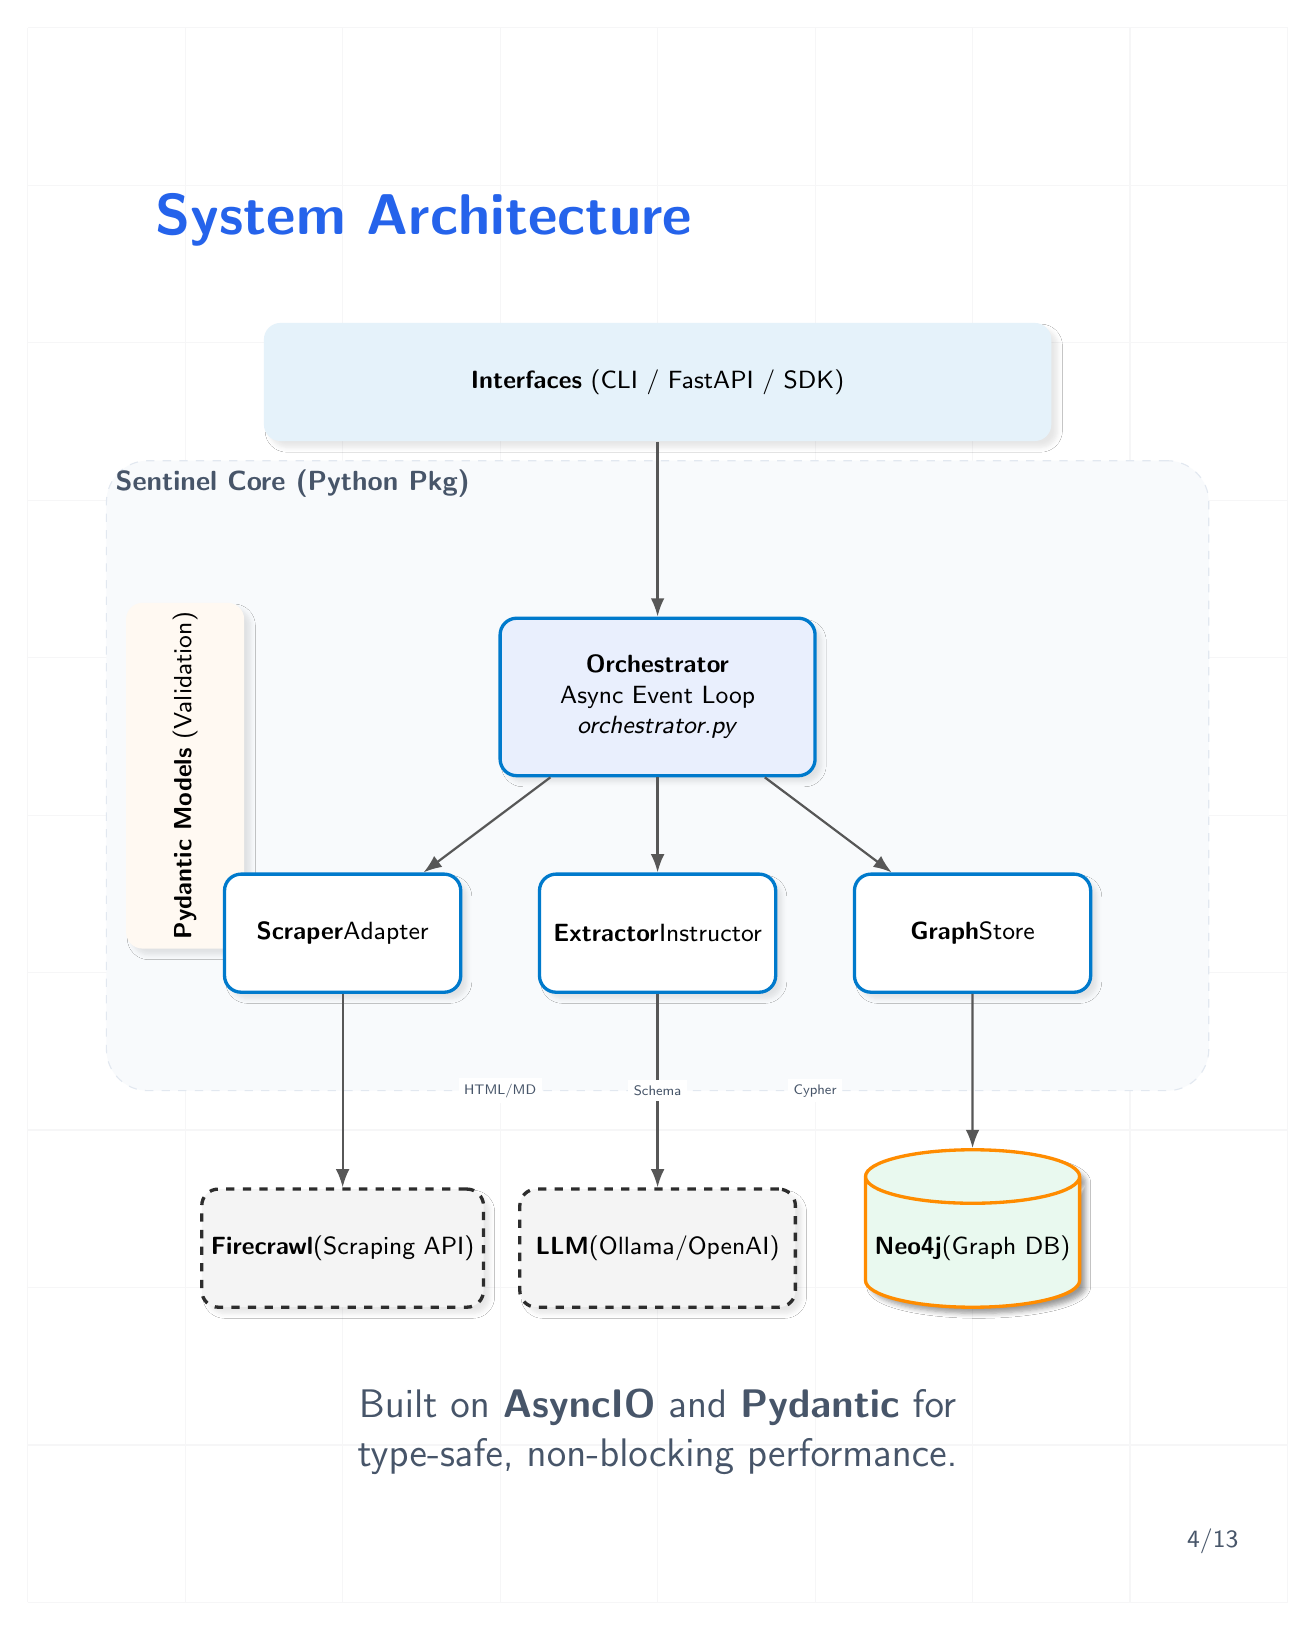
\begin{tikzpicture}
    \useasboundingbox (0,0) rectangle (\slideW, \slideH);
    \node[slide] at (0,0) {};
    \draw[step=2cm, textGray!5, thin] (0,0) grid (\slideW, \slideH);
    
    \node[h2] at (\margin, 18) {System Architecture};
    
    \begin{scope}[shift={(8, 10)}]
        % Background Container for Core
        \node[rectangle, rounded corners=15pt, fill=bgOffWhite, draw=borderGray, dashed, minimum width=14cm, minimum height=8cm] (container) at (0, 0.5) {};
        \node[anchor=north west, text=textGray, font=\bfseries] at (container.north west) {Sentinel Core (Python Pkg)};

        % 1. Interfaces (Top)
        \node[basic, fill=archPrimary!10, minimum width=10cm] (api) at (0, 5.5) {\textbf{Interfaces} (CLI / FastAPI / SDK)};
        
        % 2. Orchestrator (Center)
        \node[module, fill=primaryBlue!10, minimum width=4cm, minimum height=2cm, align=center] (orch) at (0, 1.5) {
            \textbf{Orchestrator}\\
            \small Async Event Loop\\
            \small \textit{orchestrator.py}
        };

        % 3. Data Models (Side)
        \node[basic, fill=archAccent!5, rotate=90, minimum width=4cm] (models) at (-6, 0.5) {\textbf{Pydantic Models} (Validation)};

        % 4. Components (Bottom of Core)
        \node[module, fill=bgWhite, minimum width=3cm] (scraper) at (-4, -1.5) {\textbf{Scraper}\\ \small Adapter};
        \node[module, fill=bgWhite, minimum width=3cm] (extract) at (0, -1.5) {\textbf{Extractor}\\ \small Instructor};
        \node[module, fill=bgWhite, minimum width=3cm] (graph) at (4, -1.5) {\textbf{Graph}\\ \small Store};

        % 5. External Infrastructure (Bottom)
        \node[external, fill=archSecondary!5] (firecrawl) at (-4, -5.5) {\textbf{Firecrawl}\\ \small (Scraping API)};
        \node[external, fill=archSecondary!5] (llm) at (0, -5.5) {\textbf{LLM}\\ \small (Ollama/OpenAI)};
        \node[database, fill=success!10] (neo4j) at (4, -5.5) {\textbf{Neo4j}\\ \small (Graph DB)};

        % Connections
        \draw[archConnector] (api) -- (orch);
        \draw[archConnector] (orch) -- (scraper);
        \draw[archConnector] (orch) -- (extract);
        \draw[archConnector] (orch) -- (graph);
        
        \draw[archConnector] (scraper) -- (firecrawl);
        \draw[archConnector] (extract) -- (llm);
        \draw[archConnector] (graph) -- (neo4j);
        
        % Data Flow Labels
        \node[font=\tiny, text=textGray, fill=bgWhite, inner sep=2pt] at (-2, -3.5) {HTML/MD};
        \node[font=\tiny, text=textGray, fill=bgWhite, inner sep=2pt] at (0, -3.5) {Schema};
        \node[font=\tiny, text=textGray, fill=bgWhite, inner sep=2pt] at (2, -3.5) {Cypher};
    \end{scope}
    
    \node[anchor=south, align=center, text=textGray, font=\Large, text width=14cm] at (8, 1.5) {
        Built on \textbf{AsyncIO} and \textbf{Pydantic} for type-safe, non-blocking performance.
    };
    
    \node[anchor=south east, text=textGray, font=\small] at (15.5, 0.5) {4/13};
\end{tikzpicture}

% =================================================================================
% SLIDE 5: DATA PIPELINE (New Added Slide)
% =================================================================================
\begin{tikzpicture}
    \useasboundingbox (0,0) rectangle (\slideW, \slideH);
    \node[slide] at (0,0) {};
    \draw[step=2cm, textGray!5, thin] (0,0) grid (\slideW, \slideH);
    
    \node[h2] at (\margin, 18) {How It Works: The Pipeline};
    \node[body] at (\margin, 16.5) {
        A robust, type-safe pipeline powered by Firecrawl, Pydantic, and Neo4j.
    };
    
    \begin{scope}[shift={(8, 9)}]
        % 1. Input
        \node[processNode, fill=bgWhite] (url) at (-6, 4) {\faGlobe\ URL};
        
        % 2. Scraper (Firecrawl)
        \node[processNode, fill=accentTeal!10, draw=accentTeal] (fire) at (-2, 4) {\textbf{Firecrawl}};
        \node[artifact, below=0.2cm of fire] (md) {\# Markdown\\\#\# Clean\\- List};
        
        % 3. Extractor (LLM)
        \node[processNode, fill=primaryBlue!10, draw=primaryBlue] (llm) at (2, 4) {\textbf{LLM Extract}};
        \node[artifact, below=0.2cm of llm] (json) {\{"nodes": [],\\"edges": []\}};
        
        % 4. Diff Engine
        \node[processNode, fill=warning!10, draw=warning] (diff) at (6, 4) {\textbf{Diff Engine}};
        \node[artifact, below=0.2cm of diff] (hash) {Hash: a1b2...\\Changed: Yes};
        
        % 5. Storage (Neo4j)
        \node[database, fill=success!10, draw=success] (db) at (0, -2) {\textbf{Neo4j}};
        
        % Connections
        \draw[connector] (url) -- (fire);
        \draw[connector] (fire) -- node[above, font=\tiny] {Markdown} (llm);
        \draw[connector] (llm) -- node[above, font=\tiny] {GraphData} (diff);
        \draw[connector] (diff) |- node[right, near start, font=\tiny] {Upsert} (db);
        
        % Annotations
        \node[text=textGray, font=\small, align=center] at (-2, 6) {\textbf{1. Scrape}\\Converts HTML\\to Markdown};
        \node[text=textGray, font=\small, align=center] at (2, 6) {\textbf{2. Structure}\\Extracts Entities\\\& Relations};
        \node[text=textGray, font=\small, align=center] at (6, 6) {\textbf{3. Verify}\\Checks Hashes\\vs Database};
        \node[text=textGray, font=\small, align=center] at (0, -5) {\textbf{4. Store}\\Temporal Graph\\(ValidFrom/To)};
    \end{scope}
    
    % Problem Solved Note
    \node[anchor=south, fill=bgOffWhite, draw=borderGray, rounded corners=6pt, inner sep=8pt] at (8, 1) {
        \small \faCheck\ \textbf{Problem Solved:} We automated this entire pipeline into a simple Python library.
    };

    \node[anchor=south east, text=textGray!50, font=\small] at (15.5, 0.5) {5/13};
\end{tikzpicture}


% =================================================================================
% SLIDE 6: SELF-HEALING LOGIC (Flowchart)
% =================================================================================
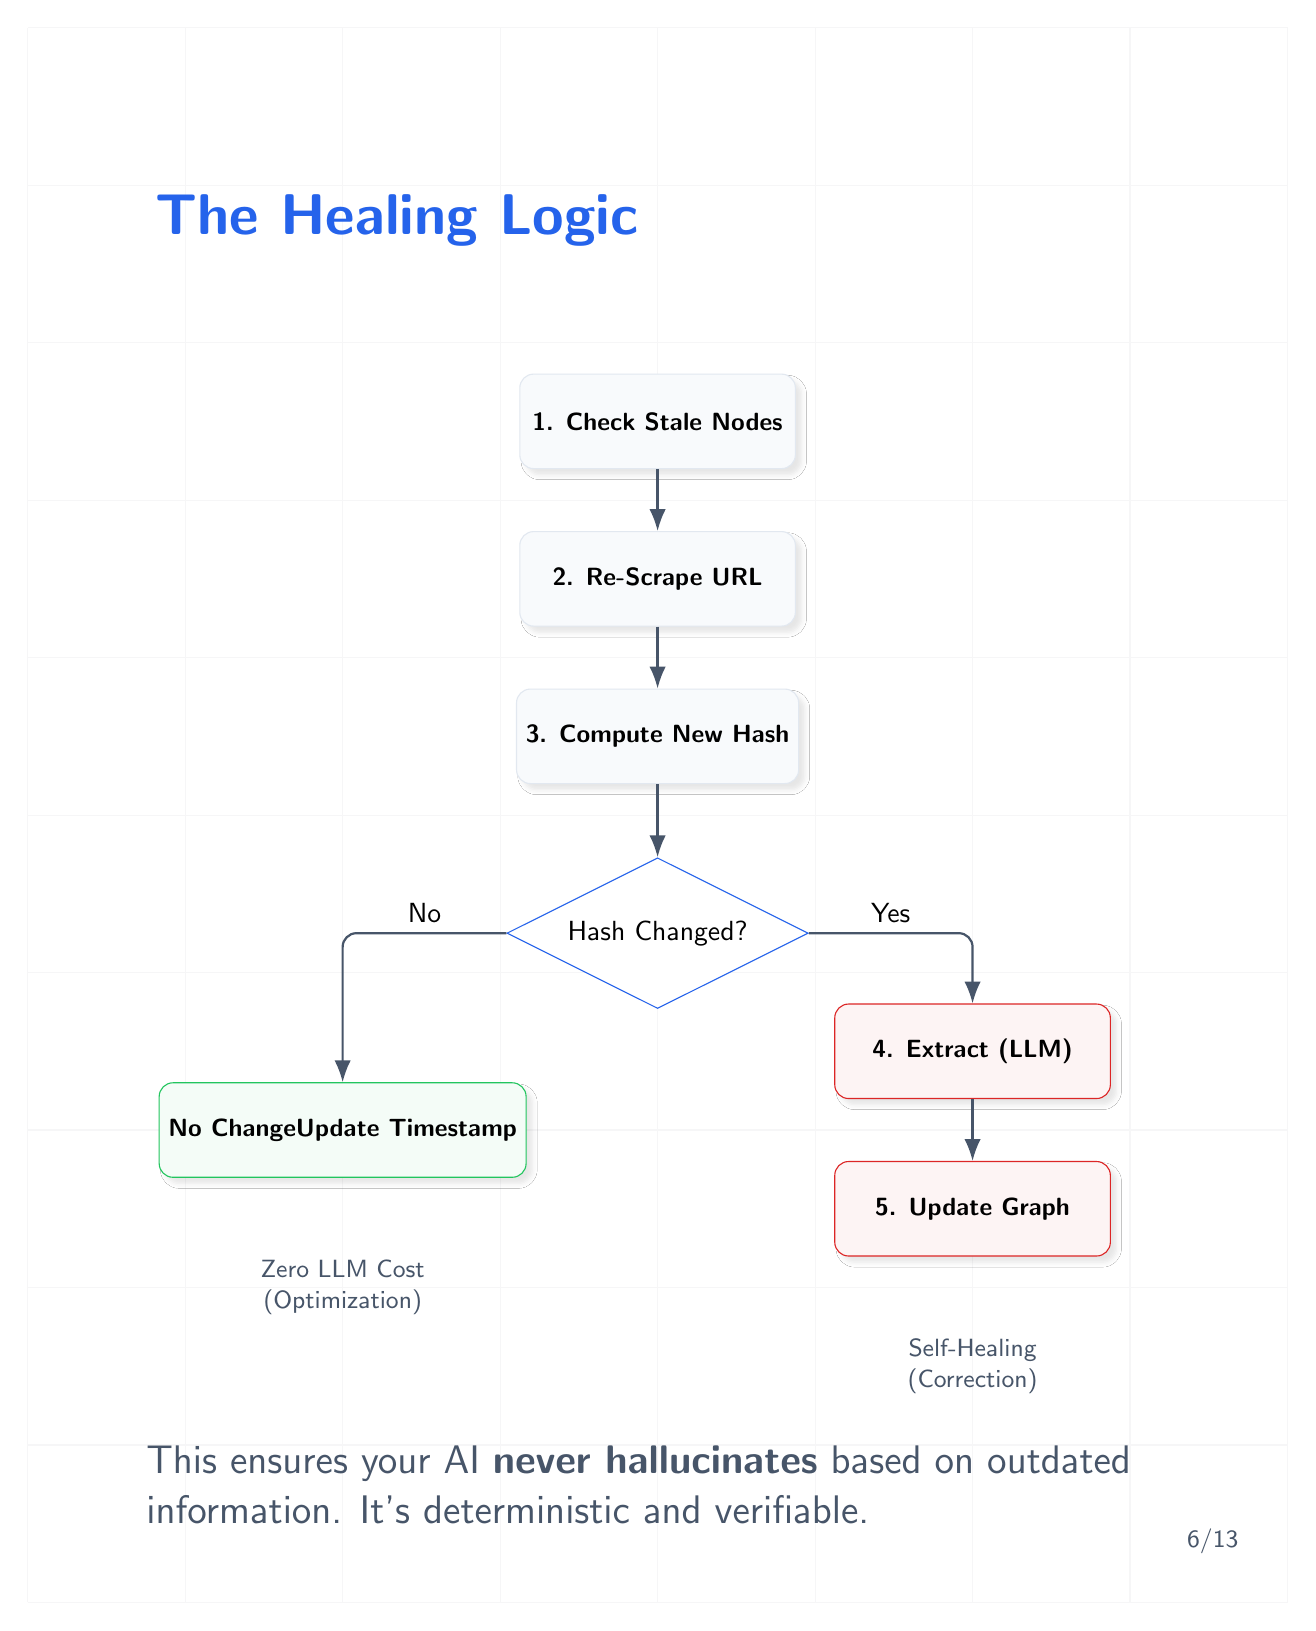
\begin{tikzpicture}
    \useasboundingbox (0,0) rectangle (\slideW, \slideH);
    \node[slide] at (0,0) {};
    \draw[step=2cm, textGray!5, thin] (0,0) grid (\slideW, \slideH);
    
    \node[h2] at (\margin, 18) {The Healing Logic};
    
    \begin{scope}[shift={(8, 10)}]
        % Flowchart
        \node[archBox, fill=bgOffWhite] (start) at (0, 5) {1. Check Stale Nodes};
        \node[archBox, fill=bgOffWhite] (scrape) at (0, 3) {2. Re-Scrape URL};
        \node[archBox, fill=bgOffWhite] (hash) at (0, 1) {3. Compute New Hash};
        
        % Decision
        \node[diamond, aspect=2, draw=primaryBlue, fill=bgWhite, text width=2.5cm, align=center] (decide) at (0, -1.5) {Hash Changed?};
        
        % No Change
        \node[archBox, draw=success, fill=success!5] (verify) at (-4, -4) {\textbf{No Change}\\Update Timestamp};
        
        % Change
        \node[archBox, draw=alertRed, fill=alertRed!5] (extract) at (4, -3) {4. Extract (LLM)};
        \node[archBox, draw=alertRed, fill=alertRed!5] (update) at (4, -5) {5. Update Graph};
        
        % Edges
        \draw[connector] (start) -- (scrape);
        \draw[connector] (scrape) -- (hash);
        \draw[connector] (hash) -- (decide);
        
        \draw[connector] (decide) -| node[near start, above] {No} (verify);
        \draw[connector] (decide) -| node[near start, above] {Yes} (extract);
        \draw[connector] (extract) -- (update);
        
        % Cost Note
        \node[text=textGray, font=\small, align=center] at (-4, -6) {Zero LLM Cost\\(Optimization)};
        \node[text=textGray, font=\small, align=center] at (4, -7) {Self-Healing\\(Correction)};
    \end{scope}
    
    \node[body, at={(\margin, 2)}] {
        This ensures your AI \textbf{never hallucinates} based on outdated information. It's deterministic and verifiable.
    };
    
    \node[anchor=south east, text=textGray, font=\small] at (15.5, 0.5) {6/13};
\end{tikzpicture}

% =================================================================================
% SLIDE 7: VISUALIZING THE HEAL (Visual Confirmation)
% =================================================================================
\begin{tikzpicture}
    \useasboundingbox (0,0) rectangle (\slideW, \slideH);
    \node[slide] at (0,0) {};
    \draw[step=2cm, textGray!5, thin] (0,0) grid (\slideW, \slideH);
    
    \node[h2] at (\margin, 18) {Visualizing the Heal};
    \node[body] at (\margin, 16.5) {
        See how Sentinel surgically updates the graph when source data changes.
    };
    
    \begin{scope}[shift={(8, 9)}]
        % Container
        \node[rectangle, rounded corners=15pt, fill=bgOffWhite, minimum width=14cm, minimum height=9cm] at (0,0) {}; % Fixed bgOffOff typo
        
        % Timeline Top (Day 1)
        \node[anchor=west, font=\bfseries\small, text=textGray] at (-6, 3) {DAY 1: INITIAL STATE};
        \node[circle, fill=bgWhite, draw=primaryBlue, minimum size=1.2cm] (s1) at (-4, 1.5) {Stripe};
        \node[rectangle, fill=bgWhite, draw=textGray, minimum width=1.5cm] (p1) at (-1, 1.5) {2.9\%};
        \draw[->, thick, textGray] (s1) -- node[above, font=\tiny] {FEES} (p1);
        \node[right, font=\tiny, text=success] at (p1.east) {Valid};

        % Timeline Bottom (Day 2)
        \node[anchor=west, font=\bfseries\small, text=textGray] at (-6, -1) {DAY 2: SOURCE UPDATE};
        \node[circle, fill=bgWhite, draw=primaryBlue, minimum size=1.2cm] (s2) at (-4, -2.5) {Stripe};
        
        % Old Node (Invalidated)
        \node[rectangle, fill=bgWhite, draw=alertRed, dashed, minimum width=1.5cm, opacity=0.6] (p2old) at (-1, -1.5) {2.9\%};
        \draw[->, dashed, alertRed, opacity=0.6] (s2) -- (p2old);
        \node[right, font=\tiny, text=alertRed] at (p2old.east) {Invalidated};
        
        % New Node (Created)
        \node[rectangle, fill=success!10, draw=success, line width=1.5pt, minimum width=1.5cm] (p2new) at (-1, -3.5) {\textbf{3.0\%}};
        \draw[->, thick, success, line width=1.5pt] (s2) -- node[below, font=\tiny] {FEES} (p2new);
        \node[right, font=\tiny, text=success] at (p2new.east) {Active (New)};
        
        % Process Flow on Right
        \node[processNode, fill=primaryBlue, text=bgWhite, minimum width=3cm] (detect) at (4, 1.5) {\faSearch\ Change Detected};
        \node[processNode, fill=bgWhite, minimum width=3cm] (extract) at (4, -0.5) {\faBrain\ LLM Extract};
        \node[processNode, fill=bgWhite, minimum width=3cm] (update) at (4, -2.5) {\faDatabase\ Graph Update};
        
        \draw[connector] (detect) -- (extract);
        \draw[connector] (extract) -- (update);
        \draw[connector, dashed] (update) -- (p2new);
    \end{scope}
    
    \node[anchor=south east, text=textGray, font=\small] at (15.5, 0.5) {7/13};
\end{tikzpicture}

% =================================================================================
% SLIDE 8: TIME TRAVEL (Unique Feature)
% =================================================================================
\begin{tikzpicture}
    \useasboundingbox (0,0) rectangle (\slideW, \slideH);
    \node[slide] at (0,0) {};
    \draw[step=2cm, textGray!5, thin] (0,0) grid (\slideW, \slideH);
    
    \node[h2] at (\margin, 18) {Feature: Time Travel};
    \node[body] at (\margin, 16.5) {
        Query your Knowledge Graph as it existed at any point in the past.
    };
    
    \begin{scope}[shift={(8, 9)}]
        % Logic Box
        \node[card, fill=bgOffWhite, minimum width=13cm, minimum height=3cm, align=left] at (0, 4) {
            \textbf{\faCode\ Temporal Edge Logic (Neo4j)}\\
            \small Every relationship in Sentinel has validity timestamps:\\
            \texttt{edge.valid\_from = <timestamp>}\\
            \texttt{edge.valid\_to = <timestamp | null>}
        };
        
        % Visual: Timeline Slider
        \draw[line width=2pt, textGray!30] (-5, 0) -- (5, 0);
        \draw[line width=2pt, primaryBlue] (-5, 0) -- (2, 0); % Active range
        \fill[primaryBlue] (2, 0) circle (6pt); % Slider Handle
        \node[above, font=\bfseries\small, text=primaryBlue] at (2, 0.3) {NOW};
        
        \fill[textGray] (-3, 0) circle (4pt);
        \node[below, font=\tiny, text=textGray] at (-3, -0.3) {Yesterday};
        
        % Graph State Visuals
        % State A (Past)
        \node[circle, fill=bgWhite, draw=textGray, opacity=0.5] (n1) at (-4, -3) {A};
        \node[circle, fill=bgWhite, draw=textGray, opacity=0.5] (n2) at (-2, -3) {B};
        \draw[->, dashed, textGray, opacity=0.5] (n1) -- node[above, font=\tiny] {Old} (n2);
        
        % State B (Present)
        \node[circle, fill=bgWhite, draw=primaryBlue] (n3) at (2, -3) {A};
        \node[circle, fill=bgWhite, draw=primaryBlue] (n4) at (4, -3) {C};
        \draw[->, thick, primaryBlue] (n3) -- node[above, font=\tiny] {New} (n4);
        
        % Arrow
        \draw[->, thick, textGray, bend left] (-1, -3) to node[above, font=\small] {Evolution} (1, -3);
    \end{scope}
    
    \node[body, at={(\margin, 2.5)}] {
        \textbf{Why?} Audit trails, compliance, and debugging. See exactly what your AI knew when it answered a user's question last week.
    };
    
    \node[anchor=south east, text=textGray, font=\small] at (15.5, 0.5) {8/13};
\end{tikzpicture}

% =================================================================================
% SLIDE 9: COMPETITOR RECON (Refined Application Slide)
% =================================================================================
\begin{tikzpicture}
    \useasboundingbox (0,0) rectangle (\slideW, \slideH);
    \node[slide] at (0,0) {};
    \draw[step=2cm, textGray!5, thin] (0,0) grid (\slideW, \slideH);
    
    \node[h2] at (\margin, 18) {Example: Competitor Analysis};
    \node[body] at (\margin, 16.5) {
        Automated surveillance of competitor websites to detect silent updates.
    };
    
    \begin{scope}[shift={(8, 9)}]
        % Background Area
        \node[rectangle, rounded corners=20pt, fill=bgOffWhite, minimum width=14cm, minimum height=8cm] at (0,0) {};
        
        % 1. Targets (Left)
        \node[anchor=south, font=\bfseries\small, text=textGray] at (-5, 2.5) {TARGET SITES};
        \node[card, minimum width=3cm, minimum height=1cm, fill=bgWhite] (c1) at (-5, 1.5) {\faGlobe\ \textbf{Stripe}};
        \node[card, minimum width=3cm, minimum height=1cm, fill=bgWhite] (c2) at (-5, 0) {\faGlobe\ \textbf{PayPal}};
        \node[card, minimum width=3cm, minimum height=1cm, fill=bgWhite] (c3) at (-5, -1.5) {\faGlobe\ \textbf{Square}};
        
        % 2. The Lens (Center)
        \node[circle, fill=primaryBlue, text=bgWhite, minimum size=2.5cm, align=center, blur shadow] (lens) at (0, 0) {\faEye\\[0.2em] \small Sentinel\\[0.2em] \small Watcher};
        
        % 3. The Dashboard (Right)
        \node[anchor=south, font=\bfseries\small, text=textGray] at (5, 2.5) {INTELLIGENCE FEED};
        \node[card, minimum width=4.5cm, minimum height=3.5cm, fill=bgWhite, align=left] (dash) at (5, 0) {
            \scriptsize\ttfamily
            \textbf{\textcolor{textBlack}{New Diffs Detected:}}\\[0.5em]
            \textcolor{textGray}{> Source: Stripe Pricing}\\
            \textcolor{alertRed}{~~- Price: 2.9\% + 30c}\\
            \textcolor{success}{~~+ Price: 3.0\% + 30c}\\[0.5em]
            \textcolor{textGray}{> Source: PayPal Landing}\\
            \textcolor{success}{~~+ Feature: "Fast Checkout"}
        };
        
        % Connections
        \draw[connector, dashed, textGray!50] (c1) -- (lens);
        \draw[connector, dashed, textGray!50] (c2) -- (lens);
        \draw[connector, dashed, textGray!50] (c3) -- (lens);
        
        \draw[connector, line width=2pt, primaryBlue] (lens) -- (dash);
    \end{scope}
    
    \node[body, at={(\margin, 3)}] {
        \textbf{Use Case:} Sentinel continuously scans target URLs. When DOM structures or content shift, it structures the diff into your graph and triggers alerts.
    };
    
    \node[anchor=south east, text=textGray, font=\small] at (15.5, 0.5) {9/13};
\end{tikzpicture}

% =================================================================================
% SLIDE 10: CODE (Library Focus)
% =================================================================================
\begin{tikzpicture}
    \useasboundingbox (0,0) rectangle (\slideW, \slideH);
    \node[slide] at (0,0) {};
    \draw[step=2cm, textGray!5, thin] (0,0) grid (\slideW, \slideH);
    
    \node[h2] at (\margin, 18) {Set and Forget};
    \node[body] at (\margin, 16.5) {Fits into existing stacks (LangChain/LlamaIndex).};
    
    % Code Block
    \node[rectangle, rounded corners=8pt, fill=codeBg, minimum width=13cm, inner sep=20pt, anchor=north west, blur shadow] at (\margin, 15) {
        \begin{minipage}{11.5cm}
            \ttfamily\color{bgWhite}
            \small
            \textcolor{textGray}{\# 1. Initialize Sentinel}\\
            \textcolor{accentTeal}{from} sentinel\_core \textcolor{accentTeal}{import} Sentinel\\
            \textcolor{accentTeal}{from} sentinel\_core.adapters \textcolor{accentTeal}{import} Neo4jAdapter\\[0.5em]
            
            s = Sentinel(\\
            \hspace*{1em}graph=Neo4jAdapter(\textcolor{primaryBlue}{"bolt://localhost..."}),\\
            \hspace*{1em}scraper=FirecrawlScraper(api\_key=\textcolor{primaryBlue}{"..."})\\
            )\\[1em]
            
            \textcolor{textGray}{\# 2. Watch a Documentation Page}\\
            \textcolor{accentTeal}{await} s.watch(\\
            \hspace*{1em}\textcolor{primaryBlue}{"https://docs.stripe.com/api"}\\
            )\\[1em]
            
            \textcolor{textGray}{\# 3. Ask (Always Fresh)}\\
            res = \textcolor{accentTeal}{await} s.ask(\textcolor{primaryBlue}{"Rate limits?"})
        \end{minipage}
    };
    
    % Library Badge
    \node[fill=accentTeal!10, text=accentTeal, rounded corners=6pt, inner sep=8pt, font=\bfseries\small, anchor=north east] at (14.5, 15) {
        \faPython\ pip install sentinel-core
    };
    
    \node[body, at={(\margin, 5)}] {
        \textbf{We built the Python library so you don't have to.} Just \texttt{pip install} and start monitoring. Sentinel handles scheduling and diffing automatically.
    };
    
    \node[anchor=south east, text=textGray, font=\small] at (15.5, 0.5) {10/13};
\end{tikzpicture}

% =================================================================================
% SLIDE 11: UNIVERSAL SCRAPING (With Use Cases)
% =================================================================================
\begin{tikzpicture}
    \useasboundingbox (0,0) rectangle (\slideW, \slideH);
    \node[slide] at (0,0) {};
    \draw[step=2cm, textGray!5, thin] (0,0) grid (\slideW, \slideH);
    
    \node[h2] at (\margin, 18) {Universal Scraping};
    \node[body] at (\margin, 16.5) {
        Turn any dynamic website into a structured Knowledge Graph.
    };

    % Why it is necessary
    \node[card, fill=bgOffWhite, text width=13cm, inner sep=10pt] at (8, 14.5) {
        \textbf{Why Firecrawl?} Modern sites use React/Vue/JS. Simple scrapers fail. Firecrawl renders the page, handles captchas, and returns \textbf{clean Markdown} optimized for LLMs.
    };

    % The Pipeline Visual
    \begin{scope}[shift={(8, 12)}]
        % Nodes
        \node[module, fill=bgWhite, minimum width=2.5cm] (url) at (-6, 0) {\faGlobe\\ \small Dynamic URL};
        \node[module, fill=accentTeal!10, minimum width=3cm] (fire) at (-2, 0) {\textbf{Firecrawl}\\ \small Scrape \& Render};
        \node[module, fill=primaryBlue!10, minimum width=3cm] (llm) at (2, 0) {\textbf{LLM}\\ \small Extract Graph};
        \node[database, fill=success!10, minimum width=2.5cm] (db) at (6, 0) {\small Neo4j};

        % Arrows
        \draw[connector] (url) -- (fire);
        \draw[connector] (fire) -- (llm) node[midway, above, font=\tiny] {Markdown};
        \draw[connector] (llm) -- (db) node[midway, above, font=\tiny] {Nodes/Edges};
    \end{scope}

    % Real-World Use Cases Grid
    \node[anchor=north west, text=primaryBlue, font=\bfseries\large] at (\margin, 9) {Real-World Scenarios:};
    
    \begin{scope}[shift={(8, 5)}]
        \matrix[row sep=0.5cm, column sep=0.5cm] {
            \node[card, text width=5.5cm, minimum height=2.5cm] {
                \textbf{\faBook\ Dynamic RAG}\\
                \small Never answer with stale API docs. Syncs with every merge/release.
            }; &
            \node[card, text width=5.5cm, minimum height=2.5cm] {
                \textbf{\faChartLine\ Market Intel}\\
                \small Track 50+ competitor pricing pages. Get alerts on specific changes.
            }; \\
            \node[card, text width=5.5cm, minimum height=2.5cm] {
                \textbf{\faGavel\ Compliance}\\
                \small Monitor government portals for new policy PDFs and updates.
            }; &
            \node[card, text width=5.5cm, minimum height=2.5cm] {
                \textbf{\faNewspaper\ Research}\\
                \small Ingest arXiv/Tech Blogs to build a realtime knowledge graph.
            }; \\
        };
    \end{scope}
    
    \node[anchor=south east, text=textGray, font=\small] at (15.5, 0.5) {11/13};
\end{tikzpicture}

% =================================================================================
% SLIDE 12: WHY DEVELOPERS NEED THIS
% =================================================================================
\begin{tikzpicture}
    \useasboundingbox (0,0) rectangle (\slideW, \slideH);
    \node[slide] at (0,0) {};
    \draw[step=2cm, textGray!5, thin] (0,0) grid (\slideW, \slideH);
    
    \node[h2] at (\margin, 18.5) {Why Developers Need This};
    \node[body] at (\margin, 17) {
        Production-grade infrastructure for reliable RAG applications.
    };
    
    \begin{scope}[shift={(8, 9)}]
        \matrix[row sep=0.5cm, column sep=0.5cm] {
            % Card 1
            \node[card, fill=bgOffWhite, text width=6cm, minimum height=3.5cm, align=left, anchor=center] {
                \textcolor{primaryBlue}{\Large \faSync}\\[0.3em]
                \textbf{\large Self-Healing Pipelines}\\[0.2em]
                \small Sentinel detects changes in docs/wikis and auto-updates the graph. \textbf{No manual re-indexing.}
            }; &
            % Card 2
            \node[card, fill=bgOffWhite, text width=6cm, minimum height=3.5cm, align=left, anchor=center] {
                \textcolor{alertRed}{\Large \faProjectDiagram}\\[0.3em]
                \textbf{\large Graph > Vectors}\\[0.2em]
                \small Knowledge Graphs preserve relationships, enabling \textbf{multi-hop reasoning} and precise answers.
            }; \\
            % Card 3
            \node[card, fill=bgOffWhite, text width=6cm, minimum height=3.5cm, align=left, anchor=center] {
                \textcolor{accentTeal}{\Large \faCode}\\[0.3em]
                \textbf{\large Type-Safe Python}\\[0.2em]
                \small Built on \textbf{AsyncIO} and \textbf{Pydantic}. Fully typed, validated, and high-performance.
            }; &
            % Card 4
            \node[card, fill=bgOffWhite, text width=6cm, minimum height=3.5cm, align=left, anchor=center] {
                \textcolor{success}{\Large \faSpider}\\[0.3em]
                \textbf{\large Universal Scraping}\\[0.2em]
                \small Powered by \textbf{Firecrawl}. Handles dynamic JS, auth walls, and complex DOMs.
            }; \\
        };
    \end{scope}
    
    \node[anchor=south east, text=textGray, font=\small] at (15.5, 0.5) {12/13};
\end{tikzpicture}

% =================================================================================
% SLIDE 13: CTA (GitHub Focus)
% =================================================================================
\begin{tikzpicture}
    \useasboundingbox (0,0) rectangle (\slideW, \slideH);
    \node[slide] at (0,0) {};
    
    % Background
    \shade[top color=bgWhite, bottom color=primaryBlue!5] (0,0) rectangle (\slideW, \slideH);
    \draw[step=2cm, textGray!5, thin] (0,0) grid (\slideW, \slideH);
    
    % Headline
    \node[h1, align=center, text width=14cm, anchor=center] at (8, 18) {
        Click on the Logo.
    };
    \node[body, align=center, anchor=center, text width=12cm] at (8, 16.5) {
        Sentinel is 100\% Open Source. Help us build the standard for autonomous knowledge graphs.
    };

    % The "Button" - GitHub Repo
    \node[card, fill=textBlack, text=bgWhite, minimum width=10cm, minimum height=3cm, blur shadow] (repo) at (8, 13) {
        \href{https://github.com/Om7035/Sentinel-The-Self-Healing-Knowledge-Graph}{
            \begin{minipage}{9cm}
                \centering
                \Huge \faGithub\ \textbf{Sentinel}\\[0.3em]
                \normalsize \faStar\ Star us on GitHub\\[0.5em]
                \scriptsize \texttt{github.com/Om7035/Sentinel...}
            \end{minipage}
        }
    };

    % Contribution List
    \node[anchor=north, text=textGray, font=\large] at (8, 10.5) {\textbf{How to Contribute:}};
    
    \matrix[row sep=0.4cm, anchor=north] at (8, 9.5) {
        \node[right, text width=10cm] {\color{primaryBlue}\faCodeBranch\ \textbf{Submit PRs}: Add new scrapers or LLM providers.}; \\
        \node[right, text width=10cm] {\color{alertRed}\faBug\ \textbf{Create Issues}: Found a bug? Let us know.}; \\
        \node[right, text width=10cm] {\color{accentTeal}\faLightbulb\ \textbf{Suggest Features}: Shape the roadmap.}; \\
    };

    % Install Command
    \node[card, fill=bgOffWhite, text=textBlack, font=\ttfamily\Large, minimum width=10cm, align=center] at (8, 5) {
        pip install sentinel-core
    };
    
    % Read Docs Link
    \node[anchor=south, align=center] at (8, 2.5) {
        \href{https://github.com/Om7035/Sentinel-The-Self-Healing-Knowledge-Graph/blob/main/README.md}{
            \textcolor{primaryBlue}{\underline{\textbf{Read the Full Documentation}}}
        }
    };
    
    \node[anchor=south east, text=textGray, font=\small] at (15.5, 0.5) {13/13};
\end{tikzpicture}

\end{document}